\section{Εισαγωγή Διαταραχών}
\subsection{Μόνιμες Διαταραχές}
\noindentΤο δυναμικό μοντέλο του αεροχήματος δεν λαμβάνει υπόψιν πιθανές 
αποκλίσεις ποu προκύπτουν κατά την κατασκευή του. Μεγέθη που επηρεάζονται από 
αυτές τις αποκλίσεις είναι η μάζα και η ροπή αδράνειας του τρικοπτέρου καθώς και 
γεωμετρικά μεγέθη που το χαρακτηρίζουν. Οι συγκεκριμένες αποκλίσεις μπορούν να 
θεωρηθούν μόνιμες εφόσον δεν επηρεάζονται από την λειτουργία του τρικοπτέρου. Τα
μεγέθη αυτά είναι η μάζα $m$, η ροπή αδράνειας $I$ καθώς και τα χαρακτηριστικά
μήκη του τρικοπτέρου $l_i, i\in \{1,\ldots,4\}$. Για την προσομοίωση τους,  
προστίθεται μία ποσοστιαία απόκλιση στην αρχική εκτίμηση των μεγεθών αυτών.
Έτσι, τα μεγέθη που προκύπτουν θα είναι
\begin{align*}
    \widehat{m} = m + p_mm  \Rightarrow \widehat{m} =& (1+p_m)m\\
    \widehat{I} = I + p_II \Rightarrow \widehat{I} =&(1+p_I)I\\
    \widehat{l_i} = m + p_{l_i}l_i  \Rightarrow \widehat{l_i} =& 
    (1+p_{l_i})l_i
\end{align*}

όπου μεταβλητή με $\,\widehat{\dot{}}\,$ συμβολίζεται η προκύπτουσα μεταβλητή 
και $p_j$ το ποσοστό απόκλισης επί της αρχικής τιμής για $j \in\{m,I,l_i\}$.

Εφαρμόζονται οι αποκλίνουσες μεταβλητές στο δυναμικό μοντέλο, με ποσοστά 
απόκλισης $p_m = 0.1, p_I = 0.2, p_{l_{i}} = 0.1$, πραγματοποιείται προσομοίωση
για βηματικές μεταβολές των μεταβλητών εξόδου του συστήματος. Οι αποκρίσεις 
παρουσιάζονται στο ακόλουθο διάγραμμα.

\begin{figure}[H]
    \centering
    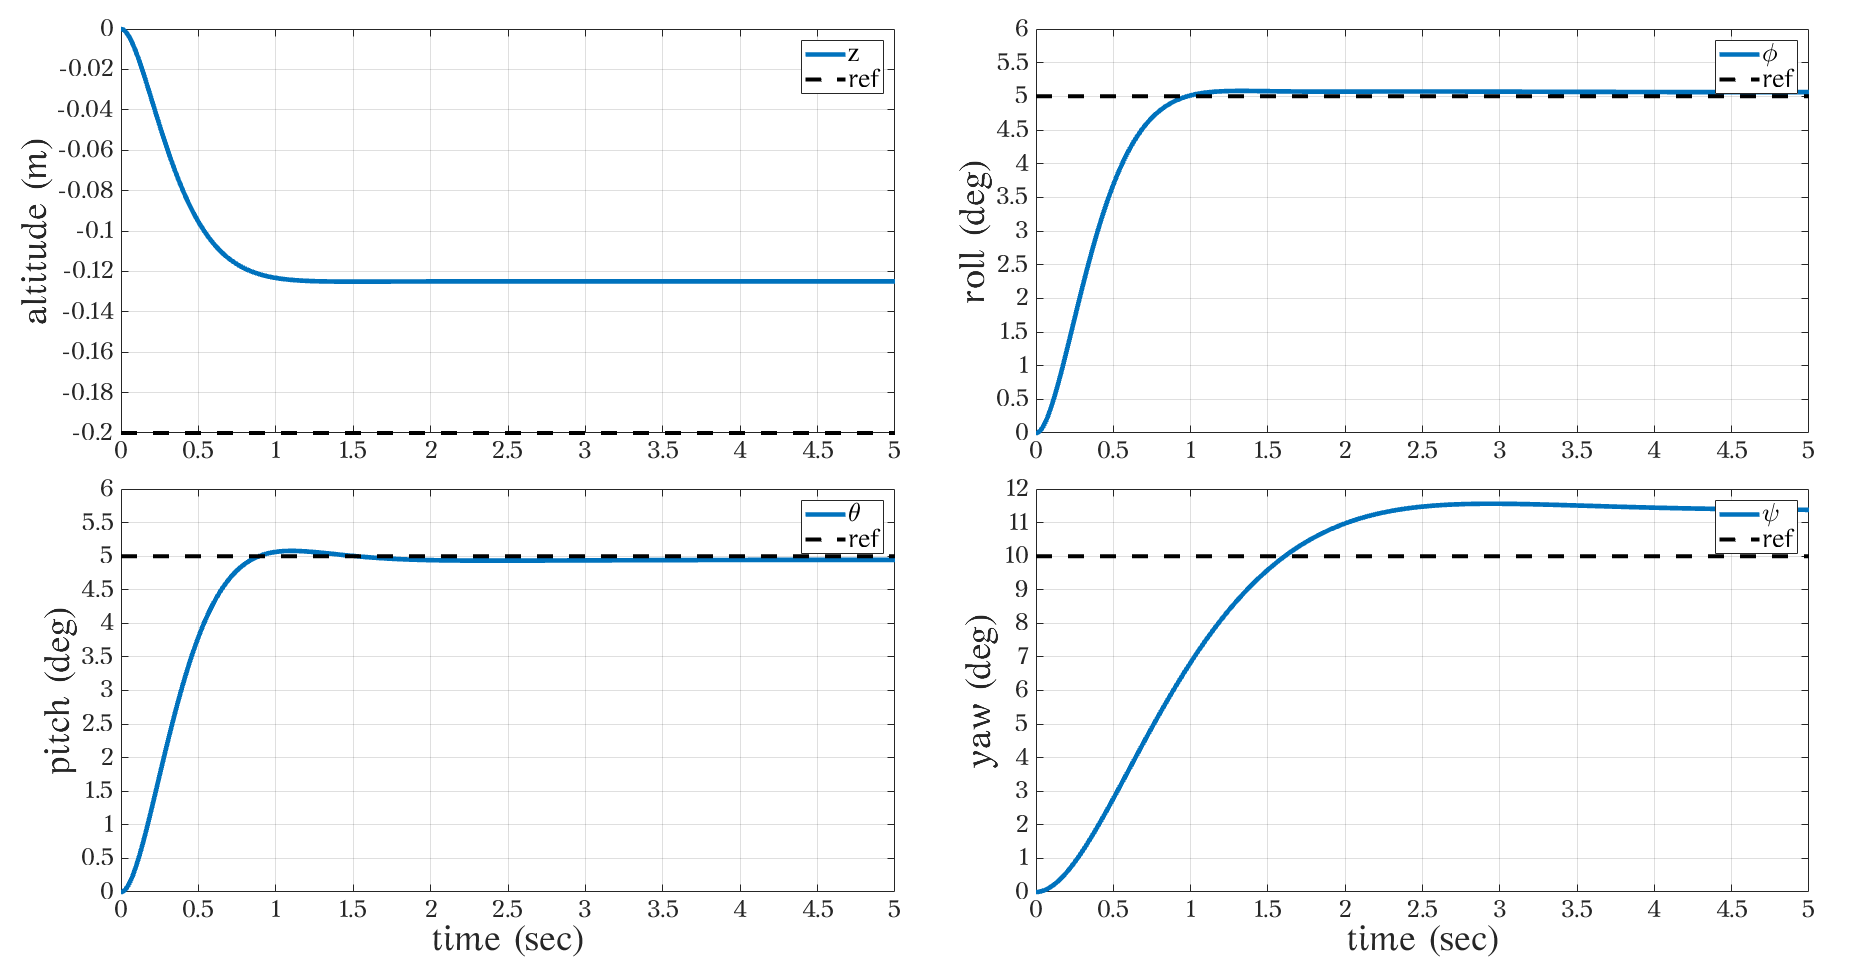
\includegraphics[width=1\textwidth]{Control/Nominal/fig_testeig_p.png}
    \caption{Βηματικές μεταβολές μεταβλητών εξόδου με μόνιμες διαταραχές.}
    \label{fig:testig}
\end{figure}

Οι δράσεις του ελεγκτή υπολογίζονται με βάση τις ονομαστικές τιμές των 
χαρακτηριστικών παραμέτρων του συστήματος. Έτσι, όταν εισάγονται διαταραχές σε 
αυτά τα μεγέθη, προκαλούνται τα μόνιμα σφάλματα που παρατηρούνται στις παραπάνω 
αποκρίσεις.

\subsection{Διαταραχές στην Έλικα}
\noindent Εκτός από τις μόνιμες διαταραχές, υπάρχουν διαταραχές που αναφέρονται 
στην πραγματική συμπεριφορά των ελίκων, όσον αφορά τα φορτία. Τέτοιες διαταραχές
προκύπτουν από την μεταβολή της πυκνότητας του αέρα ως προς το υψόμετρο πτήσης 
καθώς και την ταχύτητα του σχετικού ανέμου ως προς την έλικα.

Στο διάγραμμα που ακολουθεί παρουσιάζεται η απόκριση του τρικοπτέρου όταν έχουν 
συμπεριληφθεί οι μη-μόνιμες διαταραχές που προκύπτουν από το μοντέλο των φορτίων
της έλικας. Δίνεται ένα αρμονικό σήμα αναφοράς στη γωνία $\phi$ και μία τιμή 
αναφοράς στο ύψος. Εισάγεται, επίσης, διαταραχή ανέμου μέτρου 2 στην κλίμακα 
\tl{Beaufort} με κατεύθυνση προς το έδαφος.

\begin{figure}[H]
    \centering
    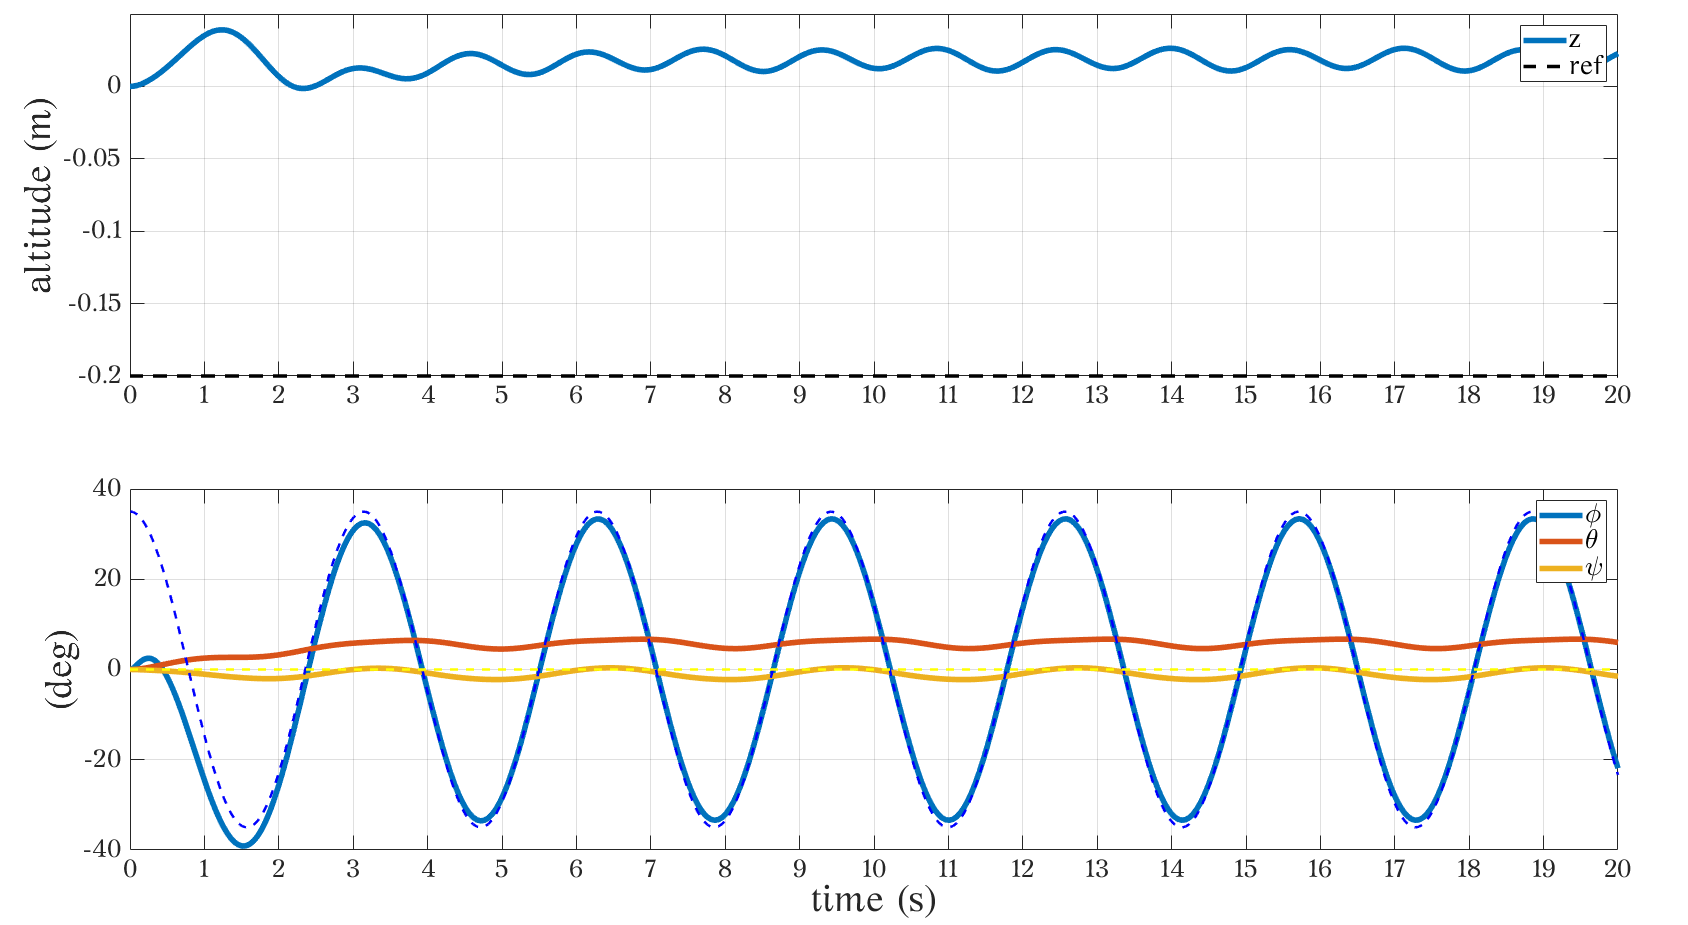
\includegraphics[width=1\textwidth]{Control/Nominal/fig_disturbance_2.png}
    \caption{Ακολούθηση σήματος αναφοράς υπό διαταραχές.}
    \label{fig:dist_1}
\end{figure}

Η ακολούθηση μιας ημιτονοειδούς καμπύλης αναφοράς στο $\phi$ επιλέχθηκε έτσι 
ώστε να φανεί η επίδραση της ταχύτητας στο μοντέλο της έλικας. Καθώς το αερόχημα
ταλαντεύεται γύρω από τον άξονα $x$, η σχετική ταχύτητα ανέμου που προσπίπτει 
κάθετα στην έλικα μεταβάλλεται αρμονικά. Έτσι, κυρίως η παραγόμενη ώθηση αλλά 
και η ροπή αντίδρασης μεταβάλλονται, γεγονός που φέρει ως αποτέλεσμα την 
ταλάντωση που βλέπουμε στην απόκριση του ύψους καθώς και την αδυναμία σύγκλισης
των υπόλοιπων γωνιών \tl{euler} στην επιθυμητή τιμή. Αξίζει να σημειωθεί ότι η 
αδυναμία σύγκλισης στην τιμή αναφοράς στο ύψος έγκειται στη υψηλή ταχύτητα 
ανέμου που δέχονται οι έλικες, καθιστώντας τες λιγότερο ισχυρές.  

Σε συνδυασμό με τα δύο προαναφερθέντα είδη διαταραχών, υπάρχει μια πληθώρα 
διαφορετικών διαταραχών που επιδρούν στο σύστημα στον πραγματικό κόσμο. 
Επιγραμματικά, η ταχύτητα του ανέμου, αποκλίσεις μετρητικών οργάνων και τα λοιπά
. Για την επίτευξη ικανοποιητικής απόδοσης του συστήματος ελέγχου, παρουσία 
διαταραχών, ο ελεγκτής πρέπει να διαθέτει την ικανότητα απόρριψης διαταραχών.